\chapter*{Übung 12}

\section*{Aufgabe 26}

Inertialsystem $\Sigma$ und Zeipunkt $t_0 = 0$: Beobachter $B$ und $B'$ an der selben Stelle. $B'$ bewegt sich mit $v$ von $B$ weg. Zum Zeitpunkt $t_1$ sind $B$ und $B'$ $\Delta s_1 = \Delta s_2$ voneinander entfernt und $B'$ dreht um. Zum Zeitpunkt $t_2$ sind $B$ und $B'$ wieder an der selben Position. 

Wir setzen $\Delta t_s = t_s - t_{s - 1}$. Es ist $\Delta s_1 = 15 \si{c \cdot a} = \Delta s_2$, $\Delta t_1 = 15 \si{a} \Delta t_2$ und $t_2 = 30 \text{ Jahre}$.

Gegeben ist, dass $v \approx c$, also $\beta = \frac{v}{c} \approx 1$ und somit $\gamma = \frac{1}{\sqrt{1 - \beta^2}} \rightarrow \infty$. Ist $\Delta t_1 = \frac{\Delta s_1}{v}$, dann ist mit Zeitdilatation\footnote{$t = \gamma \tau$} $\Delta t_1' = \frac{1}{\gamma} \Delta t_1$. Weiter ist $\Delta t_2 = \frac{\Delta s_2}{v} = \frac{\Delta s_1}{v}$ und $\Delta t_2' = \frac{1}{\gamma} \Delta t_1$. Da $t_2' = \Delta t_1' + \Delta t_2' = \frac{2 \Delta s_1}{\gamma v}$ folgt
$t_2' = \lim_{\gamma \rightarrow \infty} \frac{2 \Delta s_1}{\gamma v} = 0$.

Jetzt ist $v = \frac{c}{2}$, also $\beta = \frac{1}{2}$ und $\gamma = \frac{1}{\sqrt{1 - 1/4}} = \frac{2}{\sqrt{3}}$. Mit der Formel von eben folgt $t_2' = \frac{\sqrt{3}}{2} \frac{2 \Delta s}{\frac{c}{2}} \approx 52 \text{ Jahre}$.


Nun betrachte Skizze \ref{fig:ueb12_aufgabe26}.

\begin{figure}[h]
	\centering
	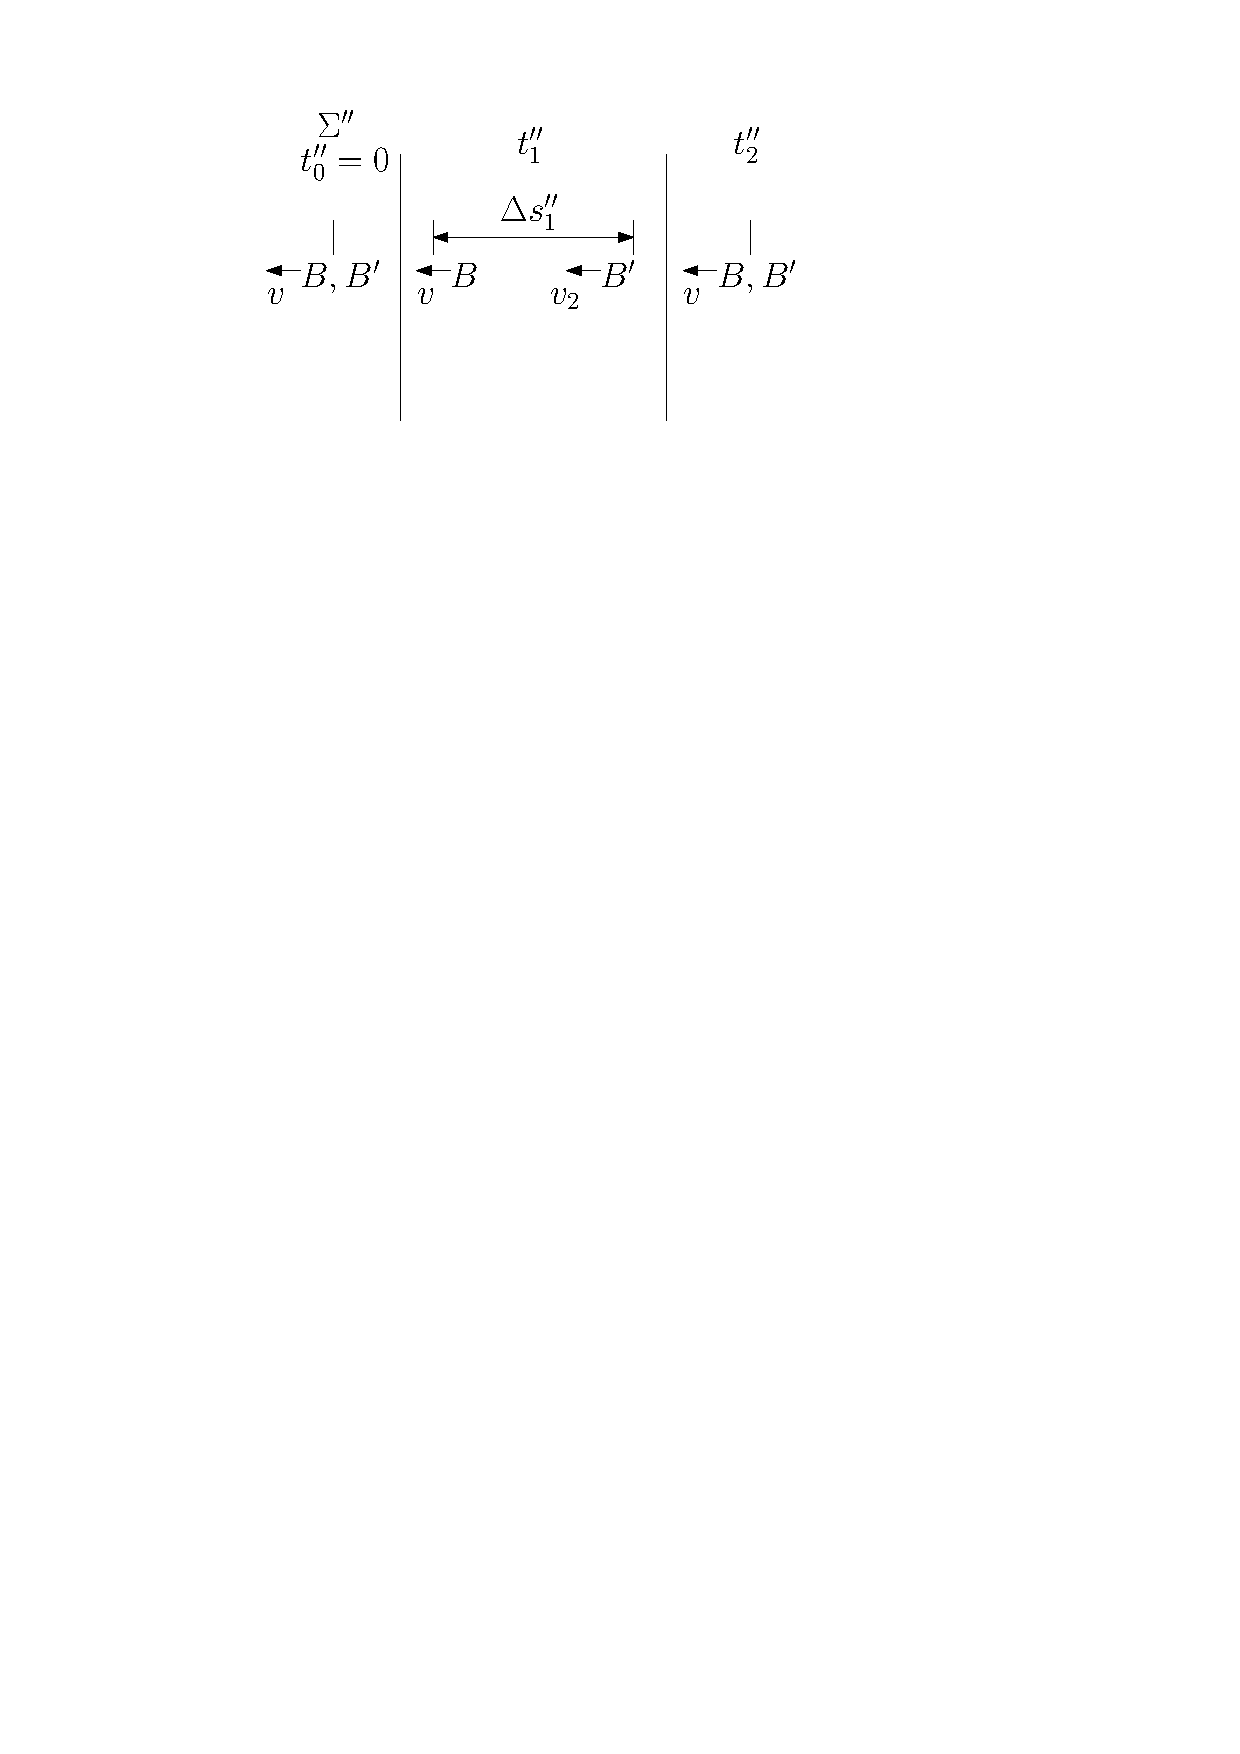
\includegraphics{figures/ueb12/aufgabe26}
	\caption{Aufgabe 26, c)}
	\label{fig:ueb12_aufgabe26}
\end{figure}

Es gilt $v_2 = \frac{v + v}{1 + \frac{v v}{c^2}} = \frac{2 v}{1 + \frac{v^2}{c^2}}$, $\beta_{v_2} = \frac{v_2}{c} = \frac{2 \beta}{1 + \beta^2}$ und 
\[
	\gamma_{v_2} = \frac{1}{\sqrt{1 - \beta^2_{v_2}}} = \frac{1}{\sqrt{1 - \frac{4 \beta^2}{(1 + \beta^2)^2}}} = \frac{1 + \beta^2}{\sqrt{(1 + \beta^2)^2 - 4 \beta^2}} 
	= \frac{1 + \beta^2}{\sqrt{(1 - \beta^2)^2}} = \frac{1 + \beta^2}{1 - \beta^2}
	\text{.}
\]

Erkenntnisse: 
\begin{enumerate}
	\item $\Delta t_1'' = \frac{1}{\gamma} \frac{\Delta s_1}{v} = \Delta t_1'$,
	\item $\Delta s_2'' = \Delta t_2'' \cdot v + \Delta s_1'' = \Delta t_2'' v_2$,
	\item $\Delta t_2'' v + \underbrace{\Delta s_1''}_{\Delta s_1 / \gamma} = \Delta t_2'' \frac{2 v}{1 + \beta^2} 
	~\Leftrightarrow~ 
	\Delta t_2'' v \left( \frac{2}{1 + \beta^2} - 1 \right) = \frac{\Delta s_1}{\gamma} 
	~\Leftrightarrow~
	\Delta t_2'' = \frac{\Delta s_1}{\gamma v} \left( \frac{2 - (1 + \beta^2)}{1 + \beta^2} \right)^{-1} = \frac{\Delta s_1}{\gamma v} \frac{1 + \beta^2}{1 - \beta^2}$,
	\item $\Delta t_2' = \frac{1}{\gamma v_2} \Delta t_2'' = \frac{1 - \beta^2}{1 + \beta^2} \frac{\Delta s_1}{\gamma v} \frac{1 + \beta^2}{1 - \beta^2} = \frac{\Delta s_1}{\gamma v}$ und schließlich
	\item $t_2' = \frac{2 \Delta s_1}{\gamma v}$.
\end{enumerate}
 
\section*{Aufgabe 27}

Eine Skizze ist auf dem Aufgabenblatt. 

\begin{description}
	\item[a)] Ein Teilchen in Ruhe mit $(m_0 c, 0, 0, 0)^T = (E / c, \vec{p})^T$ wird in $z$-Richtung geboostet:
	\[
		\begin{pmatrix}
			\gamma & - \beta \gamma & 0 & 0 \\
			- \beta \gamma & \gamma & 0 & 0 \\
			0 & 0 & 1 & 0 \\
			0 & 0 & 0 & 1
		\end{pmatrix}
		\mvec{m_0 c^2 \\ 0 \\ 0 \\ 0}
		= \mvec{\gamma m_0 c \\ - \beta \gamma m_0 c \\ 0 \\ 0} \text{,}
	\]
	also ist $E = mc^2 = \gamma m_0 c^2$. Die effektive Masse ist $m = \gamma m_0$.
	
	\item[b)] Die Energie-Impuls-Erhaltung schreibt man wie folgt auf (wobei $\vec{p}_e = \vec{0}$):
	\[
		\mvec{\frac{E_\gamma}{c} \\ \vec{p}_\gamma} + \mvec{\frac{E_e}{c} \\ \vec{p}_e}
		\overset{!}{=} \mvec{\frac{E_e'}{c} \\ \vec{p}\,'_e} + \mvec{\frac{E_\gamma'}{c} \\ \vec{p}\,'_\gamma} 
		\text{.}
	\]
	Also muss 
	\begin{enumerate}
		\item $p_\gamma + p_e = p'_\gamma + p'_e ~\Longrightarrow~ p'_e = p_\gamma + p_e - p'_\gamma$ und 
		\item $p^{'2}_e = p_\gamma^2 + p^{'2}_\gamma + p^{'2}_e + 2 (p_\gamma - p'_\gamma) p_e - 2 p_\gamma p'_\gamma$.
	\end{enumerate}
	
	Aus 2. folgt weiter 
	\begin{align*}
		& p^{'2}_\gamma = p^2_\gamma = 0 = \frac{E^2_\gamma}{c^2} - \mabs{\vec{p}_\gamma}^2 \\
		\Longleftrightarrow~& \vec{p}^2_\gamma = \frac{E^2_\gamma}{c^2} \text{,} \\
		& p^2_e = m^2_e c^2 = p^{'2}_e \text{,} \\
		& m^2_e c^2 = m_e^2 c^2 + 2(E_\gamma - E'_\gamma) E_e \frac{1}{c^2} - 2 (E_\gamma E'_\gamma \frac{1}{c^2} - \vec{p}_\gamma \vec{p}\,'_\gamma) \text{,} \\
		& \vec{p}_\gamma \vec{p}\,'_\gamma = \mabs{\vec{p}_\gamma} \mabs{\vec{p}\,'_\gamma} \cos \Theta_\gamma = \frac{E_\gamma E'_\gamma}{c^2} \cos \Theta_\gamma \\
		\Longleftrightarrow~& 0 = (E_\gamma - E'_\gamma) m_e c^2 - E_\gamma E'_\gamma (1 - \cos \Theta_\gamma) \\
		\Longleftrightarrow~& E'_\gamma (m_e c^2 + E_\gamma (1 - \cos \Theta_\gamma)) = E_\gamma m_e c^2 \\
		\Longleftrightarrow~& E'_\gamma = \frac{E_\gamma}{1 + \frac{E_\gamma}{m_e c^2} (1 - \cos \Theta_\gamma)} \text{.}
	\end{align*}

	\item[c)] Erinnerung: $E_\gamma = \frac{2 \pi \hbar c}{\lambda} = \frac{h c}{\lambda}$ und $\lambda = \frac{h}{\mabs{\vec{p}_\gamma}} = \frac{hc}{E_\gamma}$. Es ist 
	\begin{align*}
		& 0 = 2 \pi \hbar c \left( \frac{1}{\lambda} - \frac{1}{\lambda'} \right) - \frac{1 - \cos \Theta}{m_e c^2} (2 \pi \hbar)^2 \frac{1}{\lambda} \frac{1}{\lambda'} c^2 \\
		\Longleftrightarrow~& \Delta \lambda = \frac{2 \pi \hbar}{m_e c} \underbrace{(1 - \cos \Theta_\gamma)}_{2 \sin^2\left( \frac{\Theta}{2} \right)} \text{.}
	\end{align*}
\end{description}